\documentclass[11pt]{article}

\usepackage{amsmath}
\usepackage{amssymb}
\usepackage{color}
\usepackage{listings}
\usepackage{xcolor}
\usepackage{graphicx}

\definecolor{codegreen}{rgb}{0,0.6,0}
\definecolor{codegray}{rgb}{0.5,0.5,0.5}
\definecolor{codepurple}{rgb}{0.58,0,0.82}
\definecolor{backcolour}{rgb}{0.95,0.95,0.92}

\lstdefinestyle{mystyle}
{
    backgroundcolor=\color{backcolour},   
    commentstyle=\color{codegreen},
    keywordstyle=\color{magenta},
    numberstyle=\tiny\color{codegray},
    stringstyle=\color{codepurple},
    basicstyle=\ttfamily\footnotesize,
    breakatwhitespace=false,         
    breaklines=true,                 
    captionpos=b,                    
    keepspaces=true,                 
    numbers=left,                    
    numbersep=5pt,                  
    showspaces=false,                
    showstringspaces=false,
    showtabs=false,                  
    tabsize=2
}

\lstset{style=mystyle}

\textwidth=6.5in
\textheight=9in
\topmargin=-0.8in
\headheight=15.75pt
\headsep=.35in
\oddsidemargin=0.0in
\evensidemargin=0.0in

\newcommand{\Complex}{\mathbb{C}}
\newcommand{\Real}{\mathbb{R}}
\newcommand{\Dpt}{D_{+t}}
\newcommand{\Dmt}{D_{-t}}
\newcommand{\Dzt}{D_{0t}}
\newcommand{\Dpx}{D_{+x}}
\newcommand{\Dmx}{D_{-x}}
\newcommand{\Dzx}{D_{0x}}
\newcommand{\Oc}{\mathcal{O}}
\newcommand{\dx}{\Delta x}
\newcommand{\dy}{\Delta y}
\newcommand{\dt}{\Delta t}
\newcommand{\dis}[3]{{#1}^{#2}_{#3}}
\newcommand{\vd}[2]{v^{#1}_{#2}}
\newcommand{\vnd}[1]{v^{n}_{#1}}
\newcommand{\bra}[1]{\left(#1\right)}
\newcommand{\jph}{j+\frac{1}{2}}
\newcommand{\jmh}{j-\frac{1}{2}}

\begin{document}
\begin{flushright}
\small{MATH-6840\\
Vignesh Ramakrishnan\\
{\bf Due: Thursday April 7, 2022}}
\end{flushright}

\begin{center}
\large{Problem Set 8}\\
\end{center}

\begin{enumerate}
  %%%%%
  %%%%%
  %%%%%
  %%%%%
  %%%%%
  \item {\color{red}(25 pts.) Consider the wave equation }
    \[
      u_{tt}=c^2u_{xx}, \qquad t >0
    \]
     {\color{red}with initial conditions $u(x,0)=f(x)$ and $u_t(x,0)=g(x)$ (boundary conditions will be added later). }
    
    \begin{enumerate}
      %%%
      %%%
      %%%
      \item {\color{blue}Derive a sixth-order accurate (in space and time) discretization of this equation using centered spatial differences and the 3-level modified equation time stepper discussed in class. Hint: Useful discretizations may be found on the 2nd page of this document.}
      \begin{align*}
          u_{tt} =& \ c^2 u_{xx} \\
          u_{tttt} =& \ c^2 \bra{u_{xx}}_{tt} = c^2 \bra{u_{tt}}_{xx} = c^4 u_{xxxx}
      \end{align*}
      This can be generalized and written as, $u_{(2j)t} = c^{(2j)}u_{(2j)x}$ where $j=1,2,3,...$
      \begin{align*}
          u_{tt} = \Dpt\Dmt\dis{u}{n}{j}- &\bra{\frac{\dt^2}{12}u_{tttt}+\frac{\dt^4}{360}u_{6t}} = \ c^2 u_{xx} \\
          \Dpt\Dmt \dis{v}{n}{j} - \frac{\dt^2}{12}u_{tttt}-\frac{\dt^4}{360}u_{6t} =& \ c^2 \frac{2\vd{n}{j+3}-27\vd{n}{j+2}+270\vd{n}{j+1}-490\vd{n}{j}+270\vd{n}{j-1}-27\vd{n}{j-2}+2\vd{n}{j-3}}{180\dx^2}
      \end{align*}
      Simplifying this with $\sigma = \frac{c\dt}{\dx}$ becomes,
      \begin{align*}
          \vd{n+1}{j}-2\vnd{j}+\vd{n-1}{j} =& \ \frac{\sigma^2}{180}\bra{2\vd{n}{j+3}-27\vd{n}{j+2}+270\vd{n}{j+1}-490\vd{n}{j}+270\vd{n}{j-1}-27\vd{n}{j-2}+2\vd{n}{j-3}} \\
          & + \frac{\dt^2}{12}c^4 u_{xxxx} + \frac{\dt^4}{360}c^6u_{6x} \\
          \vd{n+1}{j}-2\vnd{j}+\vd{n-1}{j} =& \ \frac{\sigma^2}{180}\bra{2\vd{n}{j+3}-27\vd{n}{j+2}+270\vd{n}{j+1}-490\vd{n}{j}+270\vd{n}{j-1}-27\vd{n}{j-2}+2\vd{n}{j-3}} \\
          & + \frac{\sigma^4}{72} \bra{-\vnd{j+3}+12\vnd{j+2}-39\vnd{j+1}+56\vnd{j}-39\vnd{j-1}+12\vnd{j-2}-\vnd{j-3}}\\
          & + \frac{\sigma^6}{360}\bra{\vnd{j+3}-6\vnd{j+2}+15\vnd{j+1}-20\vnd{j}+15\vnd{j-1}-6\vnd{j-2}+\vnd{j-3}} \\
          & j=0,1,2,\ldots \ldots N
      \end{align*}
      %%%
      %%%
      %%%
      \item{\color{blue} Using Fourier mode analysis, derive an expression for the amplification factors. Create a surface plot of the magnitude of each of the two roots for $\sigma=c\Delta t/\Delta x\in[-1.1,1.1]$ and for the discrete wave number $\xi\in[-\pi,\pi]$.}\\
      Let $\vnd{j} = a^n e^{ikxj}$. Then, 
      \begin{align*}
          a-2+\frac{1}{a}=& \ \frac{\sigma^2}{180}\bra{2e^{3ikx}-27e^{2ikx}+270e^{ikx}-490+270e^{-ikx}-27e^{-2ikx}+2e^{-3ikx}}\\
          & + \frac{\sigma^4}{72} \bra{-e^{3ikx}+12e^{2ikx}-39e^{ikx}+56-39e^{-ikx}+12e^{-2ikx}-e^{-3ikx}} \\
          & + \frac{\sigma^6}{360}\bra{e^{3ikx}-6e^{2ikx}+15e^{ikx}-20+15e^{-ikx}-6e^{-2ikx}+e^{-3ikx}}
      \end{align*}
      \begin{align*}
          \frac{a^2-2a+1}{a} =& \ \frac{\sigma^2}{180}\bra{4\cos{\bra{3kx}} -54\cos{(2kx)}+ 540\cos{(kx)}-490} \\
          & + \frac{\sigma^4}{72}\bra{-2\cos{(3kx)}+24\cos{(2kx)}-78\cos{(kx)}+56} \\
          & + \frac{\sigma^6}{360}\bra{2\cos{(3kx)}-12\cos{(2kx)}+30\cos{(kx)}-20}
      \end{align*}
      Simplifying this equation it becomes,
      \begin{align*}
          a^2-2a+1 =& \ 2a \left\{\bra{\frac{\sigma^2}{90}-\frac{\sigma^4}{72}+\frac{\sigma^6}{360}}\cos{(3\xi)} + \bra{\frac{-3\sigma^2}{20} + \frac{12\sigma^4}{72}-\frac{6\sigma^6}{360}}\cos{(2\xi)}\right\}+ \\ 
          & 2a\left\{ \bra{\frac{270\sigma^2}{180}-\frac{39\sigma^4}{72}+\frac{15\sigma^6}{360}}\cos{(\xi)}+ \bra{\frac{-245\sigma^2}{180}+\frac{28\sigma^4}{72}-\frac{\sigma^6}{36}}\right\}
      \end{align*}
      Here, $\xi = kx$ and this equation can be clubbed and written as $a^2-2b+1=0$ and $a=b\pm \sqrt{b^2-1}$. The plots of the magnitude of the amplitude $|a|$ can be seen in Fig~
      %%%
      %%%
      %%%
      \item {\color{blue} Now restrict consideration to the finite domain $x\in[-1,1]$ with boundary conditions $u_x(-1,t) = \alpha(t)$, $u(1,t) = \beta(t)$. Using the computational grid defined by $x_j=-1+j\Delta x$, $0 \le j \le N$, $\Delta x=2/N$, introduce ghost cells as needed and define appropriate compatibility boundary conditions suitable for 6th order accuracy. }\\
      If 3 ghost points are introduced at either ends of the boundary, then the boundary condition at the right is given as,
      \begin{align*}
          u(1,t) =& \ \beta(t) \\
          u_{tt}(1,t) =& \ \beta_{tt}(t) \\
          c^2 u_{xx}(1,t) =& \ \beta_{tt}(t) & \text{Equation 1} \\
          c^4 u_{xxxx}(1,t) =& \ \beta_{tttt}(t) & \text{Equation 2}\\
          c^6 u_{6x}(1,t) =& \ \beta_{6t}(t) & \text{Equation 3} \\
      \end{align*}
      This using the discretization available can be written as,
      \begin{align*}
          c^2 \frac{2\vd{n}{N+3}-27\vd{n}{N+2}+270\vd{n}{N+1}-490\vd{n}{N}+270\vd{n}{N-1}-27\vd{n}{N-2}+2\vd{n}{N-3}}{180\dx^2} =& \ \beta_{tt}(t) & (1) \\
          c^4 \frac{-\vnd{N+3}+12\vnd{N+2}-39\vnd{N+1}+56\vnd{N}-39\vnd{N-1}+12\vnd{N-2}-\vnd{N-3}}{6\dx^4} =& \ \beta_{tttt}(t) & (2)\\
          c^6 \frac{\vnd{N+3}-6\vnd{N+2}+15\vnd{N+1}-20\vnd{N}+15\vnd{N-1}-6\vnd{N-2}+\vnd{N-3}}{\dx^6} =& \ \beta_{6t}(t) & (3)
      \end{align*}
      This leads to a system of Linear equations to solve for $\vnd{N+1},\vnd{N+2},\vnd{N+3}$. \\
      \begin{align*}
          \begin{bmatrix}
                2 & -27 & 270 \\
                -1 & 12 & -39 \\
                1 & -6  & 15
          \end{bmatrix} 
          \begin{bmatrix}
                \vnd{N+3}\\
                \vnd{N+2}\\
                \vnd{N+1}
          \end{bmatrix}=
          \begin{bmatrix}
                \frac{180\dx^2}{c^2}\beta_{tt}(t)+490\vnd{N}-270\vnd{N-1}+27\vnd{N-2}+2\vnd{N-3}\\
                \frac{6\dx^4}{c^4}\beta_{4t}(t) -56\vnd{N}+39\vnd{N-1}-12\vnd{N-2}+\vnd{N-3}\\
                \frac{\dx^6}{c^6}\beta_{6t}(t)+20\vnd{N}-15\vnd{N-1}+6\vnd{N-2}-\vnd{N-3}
          \end{bmatrix}
      \end{align*}
      Now similarly for the left boundary condition, 
      \begin{align*}
          u_x(-1,t) =& \ \alpha(t) & \text{Equation 4} \\
          \bra{u_{tt}}_x(-1,t) = c^2 u_{xxx}(-1,t) =& \ \alpha_{tt}(t) & \text{Equation 5} \\
          \bra{u_{4t}}_x(-1,t) = c^4 u_{5x}(-1,t) =& \ \alpha_{5t}(t) & \text{Equation 6} 
      \end{align*}
      Using the discretization available, it can be rewritten as,
      \begin{align*}
          \frac{\vnd{3}-9\vnd{2}+45\vnd{1}-45\vnd{-1}+9\vnd{-2}-\vnd{-3}}{60\dx} =& \ \alpha(t) & (4) \\
          \frac{-\vnd{3}+8\vnd{2}-13\vnd{1}+13\vnd{-1}-8\vnd{-2}+\vnd{-3}}{8\dx^3}=& \ \alpha_{tt}(t) & (5) \\
          \frac{\vnd{3}-4\vnd{2}+5\vnd{1}-5\vnd{-1}+4\vnd{-2}-\vnd{-3}}{2\dx^5}=& \ \alpha_{4t}(t) & (6)
      \end{align*}
      This is a system of linear equations which can be written as, 
      \begin{align*}
          \begin{bmatrix}
                -45 & 9 & -1\\
                13 & -8 & 1 \\
                -5 & 4  & -1
          \end{bmatrix}
          \begin{bmatrix}
                \vnd{-1} \\
                \vnd{-2} \\
                \vnd{-3}
          \end{bmatrix}=
          \begin{bmatrix}
                60\dx \alpha(t) -\vnd{3}+9\vnd{2}-45\vnd{1} \\
                \frac{8\dx^3}{c^2}\alpha_{tt}(t)+\vnd{3}-8\vnd{2}+13\vnd{1} \\
                \frac{2\dx^5}{c^4}\alpha_{4t}(t)-\vnd{3}+4\vnd{2}-5\vnd{1}
          \end{bmatrix}
      \end{align*}
      %%%
      %%%
      %%%
      \item {\color{blue}Write a code implementing the sixth-order method. Perform a convergence study using the exact solution $u(x,t)=\sin(5(x-ct))+\cos(2(x+ct))$ with $c=.9$.}\\
      It is important to find forcing first for this solution.
      \begin{align*}
          u_{tt} =& c^2 u_{xx} + F(x,t)\\
      \end{align*}
      But for this exact solution Forcing $F(x,t)=0$. 
      For $t=0$,
      \begin{align*}
          u(x,0) =& \ \sin{5x} + \cos{2x} = f(x) \\
          u_t(x,0) =& \ -5c\cos(5x)-2c\sin{2x} = g(x) \\
          u_x(-1,t) =& \ 5\cos{(-5-5ct)}-2\sin{(-2+2ct)} = \alpha(t) \\
          u(1,t) =& \ \sin{(5-5ct)} + \cos{(2+2ct)} = \beta(t)
      \end{align*}
      Now, $\alpha_{tt}(t), \alpha_{4t}(t), \beta_{tt}(t), \beta_{4t}(t), \beta_{6t}(t)$ are all computed analytically and then the boundary conditions are set.
      \lstinputlisting[caption={Wave Equation - 6th order scheme}, label={lst:O6_HE},language=Matlab]{WaveEqn1DOrder6.m}
      The convergence analysis of this scheme is displayed in Figure~\ref{fig:Q1_Err}.
      \begin{figure}[htp]
      	\centering
	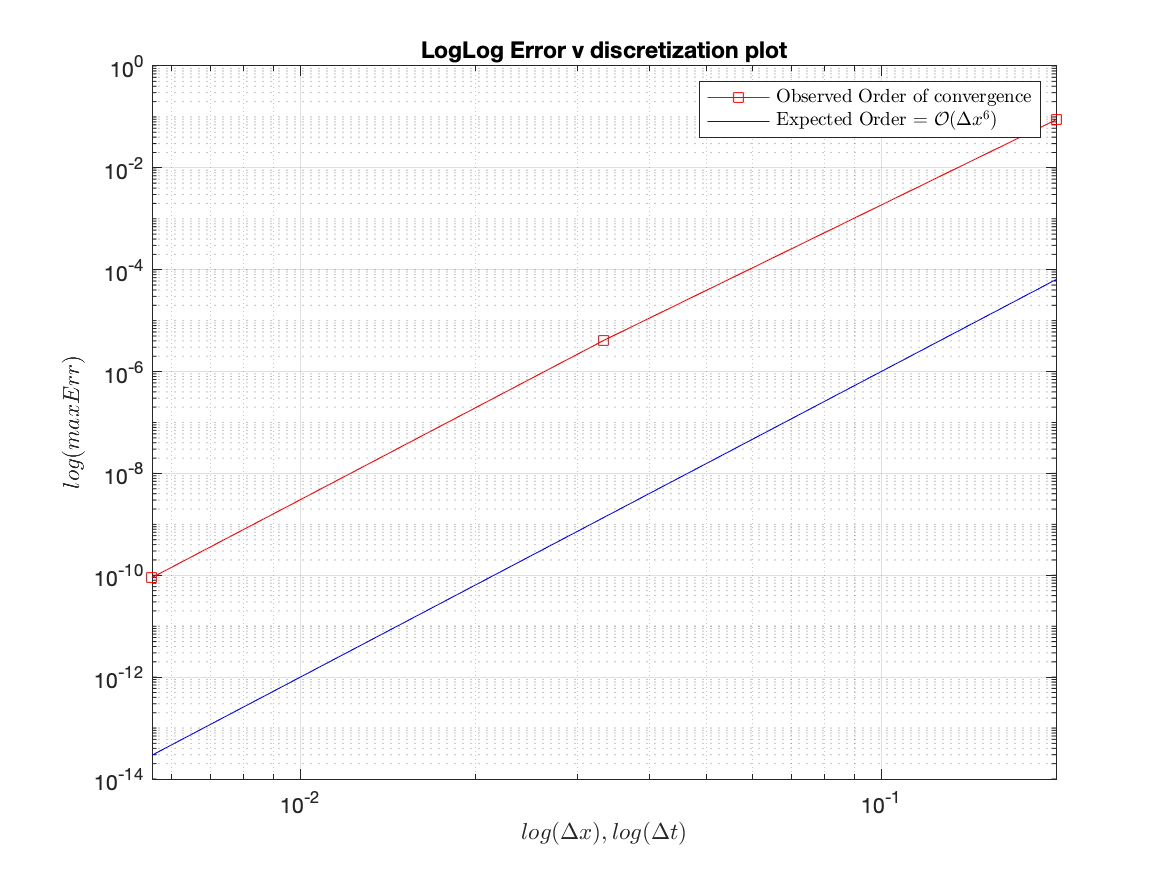
\includegraphics[width=4in]{Q1_ErrPlot.png}
	\caption{Order of Convergence}
	\label{fig:Q1_Err}
      \end{figure}
      \end{enumerate}

  %%%%%
  %%%%%
  %%%%%
  %%%%%
  %%%%%
  \item {\color{red}(25 pts.) Consider the wave propagation problem in an annular section}
    \[
      u_{tt} = c^2\left[\frac{1}{r}(ru_r)_r+\frac{1}{r^2}u_{\theta\theta}\right], \quad \frac{1}{2}<r<1, \quad -\frac{\pi}{2}<\theta<\frac{\pi}{2}, \quad t>0
    \]
    {\color{red}with initial condition $u(r,\theta,0)=f(r,\theta)$, $u_t(r,\theta,0)=g(r,\theta)$, and boundary conditions}
    \begin{align*}
      u\left(\frac{1}{2},\theta,t\right) = 0, \qquad & u_r\left(1,\theta,t\right) = 0 \\
      u\left(r,-\frac{\pi}{2},t\right) = 0 \qquad & u_{\theta}\left(r,\frac{\pi}{2},t\right) = 0.
    \end{align*}
    
    \begin{enumerate}
      %%%
      %%%
      %%%
      \item {\color{blue}Write a second-order accurate code to solve this problem using centered differencing and the 3-level modified equation time stepper discussed in class. That is to say you must to treat this as a variable coefficient operator rather than performing a chain rule (e.g. you must discretize $(ru_r)_r$ as it sits and {\bf not} convert it to $u_r+ru_{rr}$). Note this code will have a maximal stable time step and your code will need to be constructed to satisfy this constraint.}\\
      If a rectangular discretization of the domain is considered, then,
      \begin{align*}
          u_{tt} =& \ c^2\bra{u_{xx} + u_{yy}} \\
          \vd{n+1}{j,k} =& \ 2\vd{n}{j,k}-\vd{n-1}{j,k} + \frac{c^2\dt^2}{\dx^2}\bra{\vnd{j+1,k}-2\vnd{j,k}+\vnd{j-1,k}} + \frac{c^2\dt^2}{\dy^2}\bra{\vnd{j,k+1}-2\vnd{j,k}+\vnd{j,k-1}}
      \end{align*}
      Let $\vnd{j,k} = a^{n}e^{ik_1xj}e^{ik_2yk}$ and substituting this above results in,
      \begin{align*}
          a-2+\frac{1}{a} =& \ \sigma_1^2\bra{e^{ik_1x}-2+e^{-ik_1x}} + \sigma_2^2\bra{e^{ik_2y}-2+e^{-ik_2y}} \\
          \frac{a^2-2a+1}{a} =& \ 2\sigma_1^2\bra{\cos{\xi}-1} + 2\sigma_2^2\bra{\cos{\eta}-1}
      \end{align*}
      Where, $\sigma_1 = \frac{c\dt}{\dx}, \sigma_2 = \frac{c\dt}{\dy}, \xi = k_1x, \eta = k_2y$.
      \begin{align*}
          a^2-2\bra{1-\sigma_1^2\bra{1-\cos{\xi}} - \sigma_2^2\bra{1-\cos{\eta}}}a + 1 =0
      \end{align*}
      Let $b = 1-\sigma_1^2\bra{1-\cos{\xi}} - \sigma_2^2\bra{1-\cos{\eta}}$.\\
      For stability $b^2\leq 1$
      \begin{align*}
          1+\sigma_1^4(1-\cos\xi)^2+&\sigma_2^4(1-\cos\eta)^2-\\
          & 2\sigma_1^2(1-\cos\xi)-2\sigma_2^2(1-\cos\eta)+\\
          & 2\sigma_1^2\sigma_2^2(1-\cos\xi)(1-\cos\eta)\leq 1
      \end{align*}
      This can be further simplified into
      \begin{align*}
          \bra{\sigma_1^2(1-\cos\xi)+\sigma_2^2(1-\cos\eta)}^2 \leq 2\bra{\sigma_1^2(1-\cos\xi)+\sigma_2^2(1-\cos\eta)}
      \end{align*}
      The maximum value of this inequality occurs at $\cos\xi=-1$ and at $\cos\eta=-1$. Then it reduces to,
      \begin{align*}
          4\bra{\sigma_1^2+\sigma_2^2}^2\leq 4\bra{\sigma_1^2+\sigma_2^2} \\
          c^2\dt^2\bra{\frac{1}{\dx^2}+\frac{1}{\dy^2}}\leq 1\\
          \dt^2 \leq \frac{1}{c^2\bra{\frac{1}{\dx^2}+\frac{1}{\dy^2}}}
      \end{align*}
      If $\dx \leq \dy$, then
      \begin{align*}
          \dt = \frac{\dx}{c\sqrt{2}}
      \end{align*}
      In our case, we choose which ever is smaller between $\Delta r$ and $r_1\Delta\theta$ and then choose $\dt = \frac{\Delta X}{c\sqrt{2.5}}$ where $\bra{\Delta X = min\bra{\Delta r, r_1\Delta\theta}}$.
      %%%
      %%%
      %%%
      \item {\color{blue}Verify the accuracy of your code using a manufactured solution. Here you should use $N_{\theta}=3N_r$ so that in physical space the grids are approximately square. Note that you will likely need to consider non-homogeneous boundary conditions since your exact solution may not satisfy the given BCs.}\\
      Let the exact solution be, $u(r,\theta,t) = \sin(\pi r)\cos{\theta}\sin(t)$. Then
      \begin{align*}
          F(r,\theta,t) = &\ u_{tt}-c^2\bra{\frac{1}{r}\bra{ru_r}_r + \frac{1}{r^2}u_{\theta\theta}}
      \end{align*}
      Boundary conditions are
      \begin{align*}
          u(\frac{1}{2},\theta,t) =& \ \cos{\theta}\sin{(t)} = \alpha_1(\theta,t)\\
          u_r(1,\theta,t) =&\ \pi\cos{\pi}\cos\theta\sin{t} = \alpha_2(\theta,t)\\
          u(r,-\frac{\pi}{2},t) =& \ \sin{(\pi r)}\cos{\frac{-\pi}{2}}\sin{t}=\alpha_3(r,t) \\
          u_\theta(r,\frac{\pi}{2},t) =& \ -\sin{(\pi r)}\sin{\frac{\pi}{2}}\sin t = \alpha_4(r,t)
      \end{align*}
      The discretization is now written as,
      \begin{align*}
      	\vd{n+1}{j,k} = \ 2\vd{n}{j,k}-\vd{n-1}{j,k} +&\frac{\sigma_1^2}{r_{j,k}}\bra{r_{\jph,k}\vnd{j+1,k}-\bra{r_{\jph,k}+r_{\jmh,k}}\vnd{j,k}+r_{\jmh,k}\vnd{j-1,k}}\\
	&+\frac{\sigma_2^2}{r_{j,k}^2}\bra{\vnd{j,k+1}-2\vnd{j,k}+\vnd{j,k-1}} \\
	&j = 0,1,2,....,N_r \\
	&k = 0,1,2,....,N_{\theta} 
      \end{align*}
      \begin{align*}
      \frac{\vnd{-1,k}+\vnd{1,k}}{2} =& \ \alpha_1(\theta,t) \\
      \frac{\vnd{N_r+1,k}-\vnd{N_r-1,k}}{2\Delta r} =& \ \alpha_2(\theta,t) \\
      \frac{\vnd{j,-1}+\vnd{j,1}}{2} =& \ \alpha_3(r,t)\\
      \frac{\vnd{j,N_\theta +1} - \vnd{j,N_\theta -1}}{2\Delta \theta} =& \ \alpha_4(r,t)
      \end{align*}
      \lstinputlisting[caption={Mesh Generation}, label={lst:mesh_2D},language=Matlab]{genMesh.m}
      \lstinputlisting[caption={Wave Equation under 2D Mapping}, label={lst:WE_2D},language=Matlab]{WaveEqn2DMapping.m}
      The error plot looked smooth to me but I could not get second order convergence for some reason. It can be found in Fig~\ref{fig:Q2_Err} \\
      \begin{figure}[htp]
      \centering
      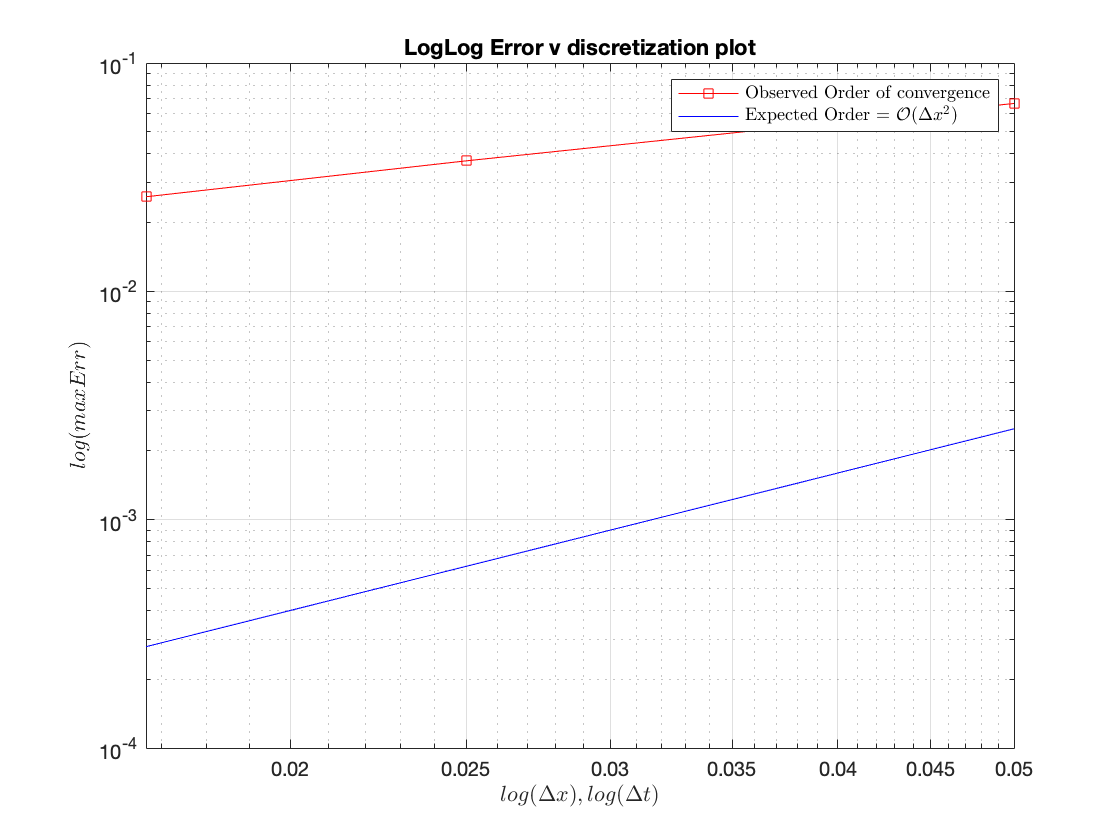
\includegraphics[width=4in]{Q2_ErrPlot.png} 
      \caption{Error Convergence plot 2D Wave Equation}
      \label{fig:Q2_Err}
      \end{figure}
      %%%
      %%%
      %%%
      \item {\color{blue}Using $c=1$, $Nr=160$ and $N_{\theta}=480$, compute numerical solutions to this problem using $f(r,\theta) = \exp(-100((r-0.75)^2+(\theta)^2))$, $g(r,\theta)=0$ at $t=0,.5,1.5,2.5$. Create surface plots of the solution for each time. In addition, create a single line plot with four curves showing the solution along the outer radius ($r=1$), as a function of $\theta$ for all four times.}\\
      The solutions are found in Fig~\ref{fig:Q2_plots} and Fig~\ref{fig:Q2_1D}.
      \begin{figure}[htp]
      \centering
      \begin{tabular}{cc}
      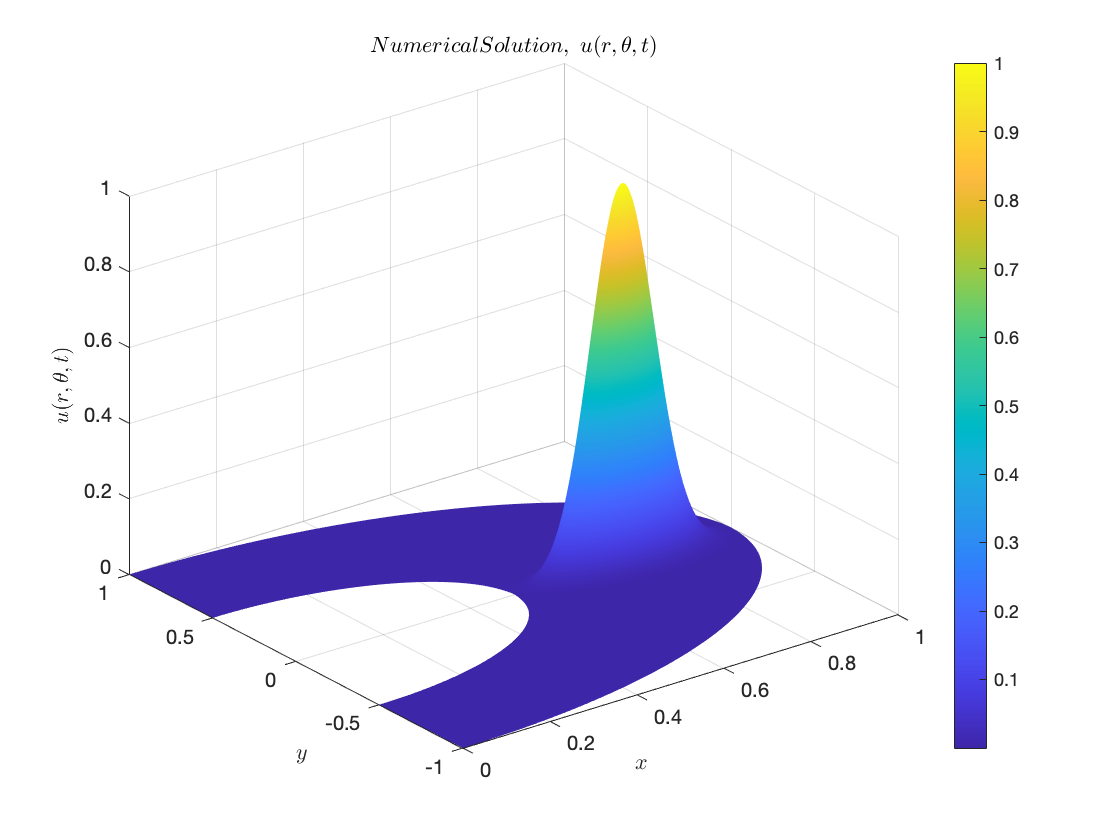
\includegraphics[width=3.5in]{Q2_t1.png} & 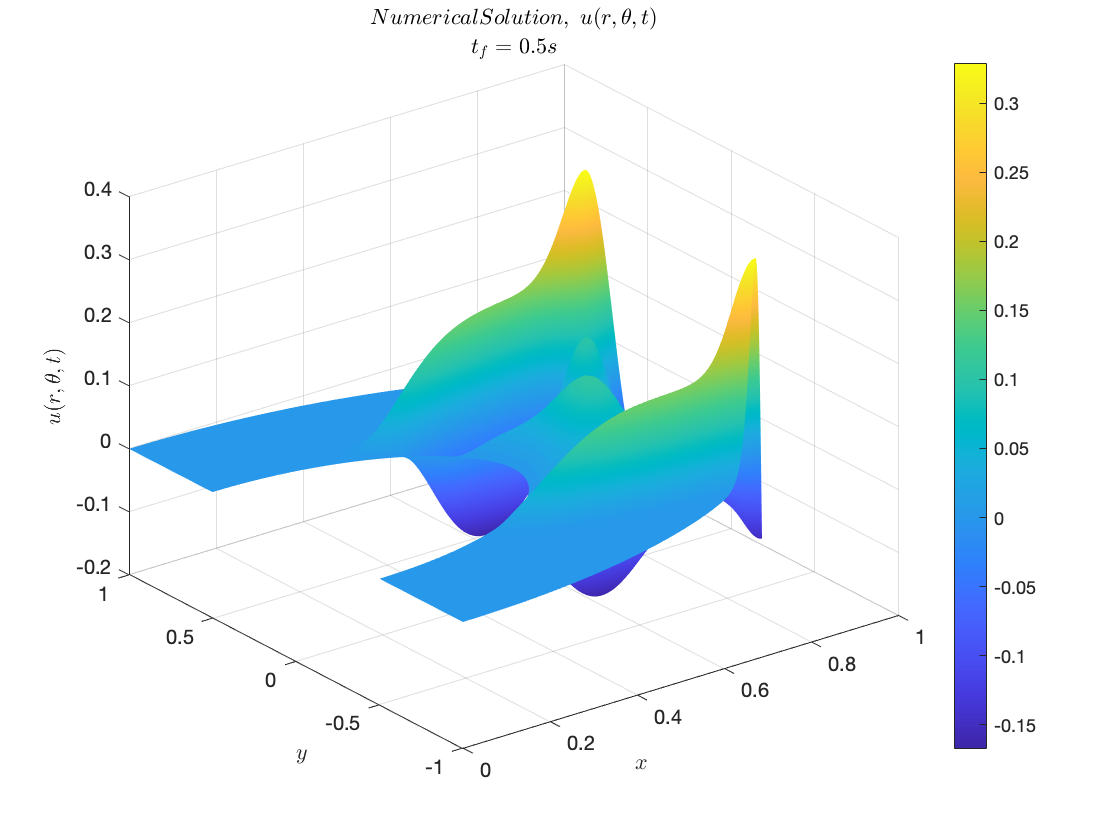
\includegraphics[width=3.5in]{Q2_t2.png} \\
      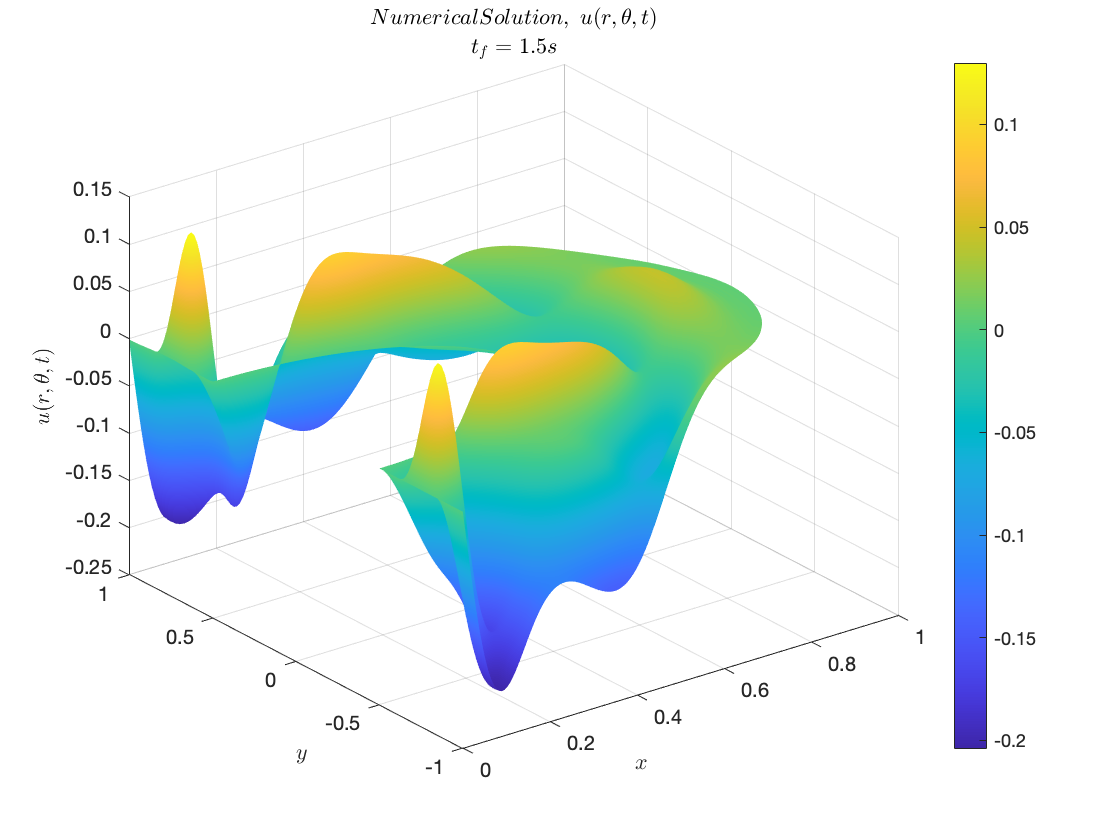
\includegraphics[width=3.5in]{Q2_t3.png} & 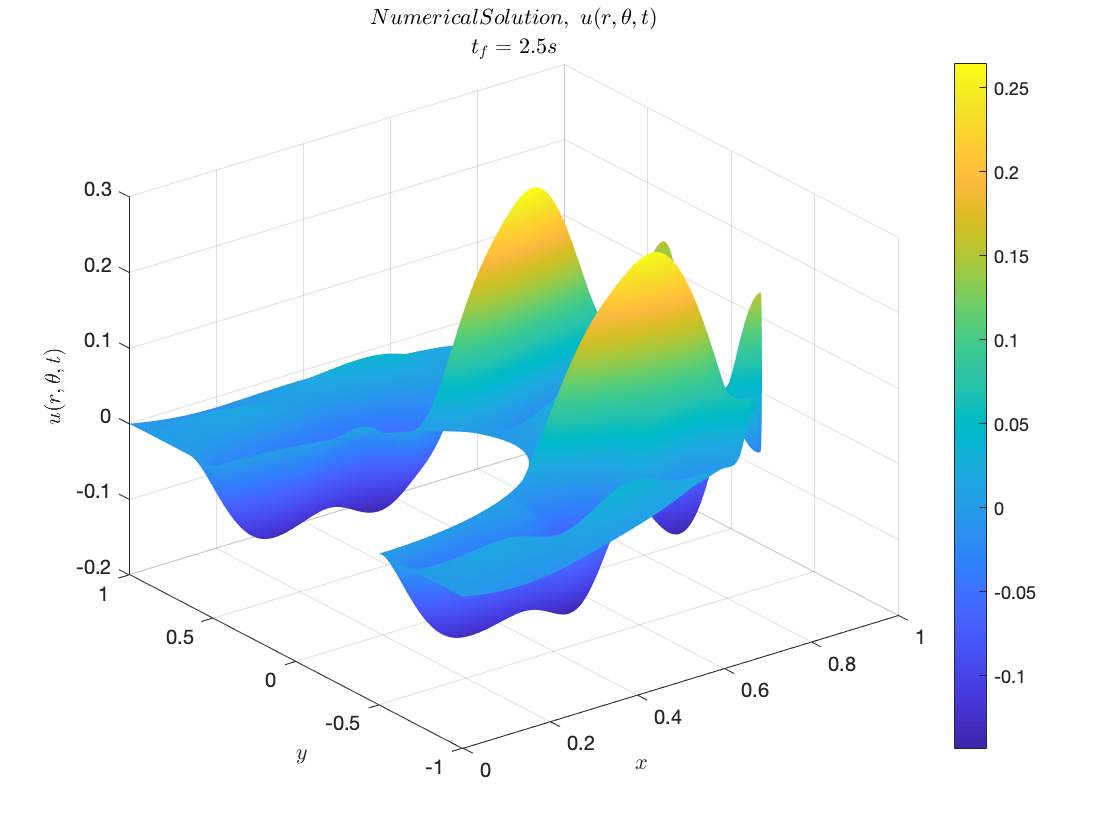
\includegraphics[width=3.5in]{Q2_t4.png}
      \end{tabular}
      \caption{Solution at different final times}
      \label{fig:Q2_plots}
      \end{figure}
      \begin{figure}[htp]
      \centering
      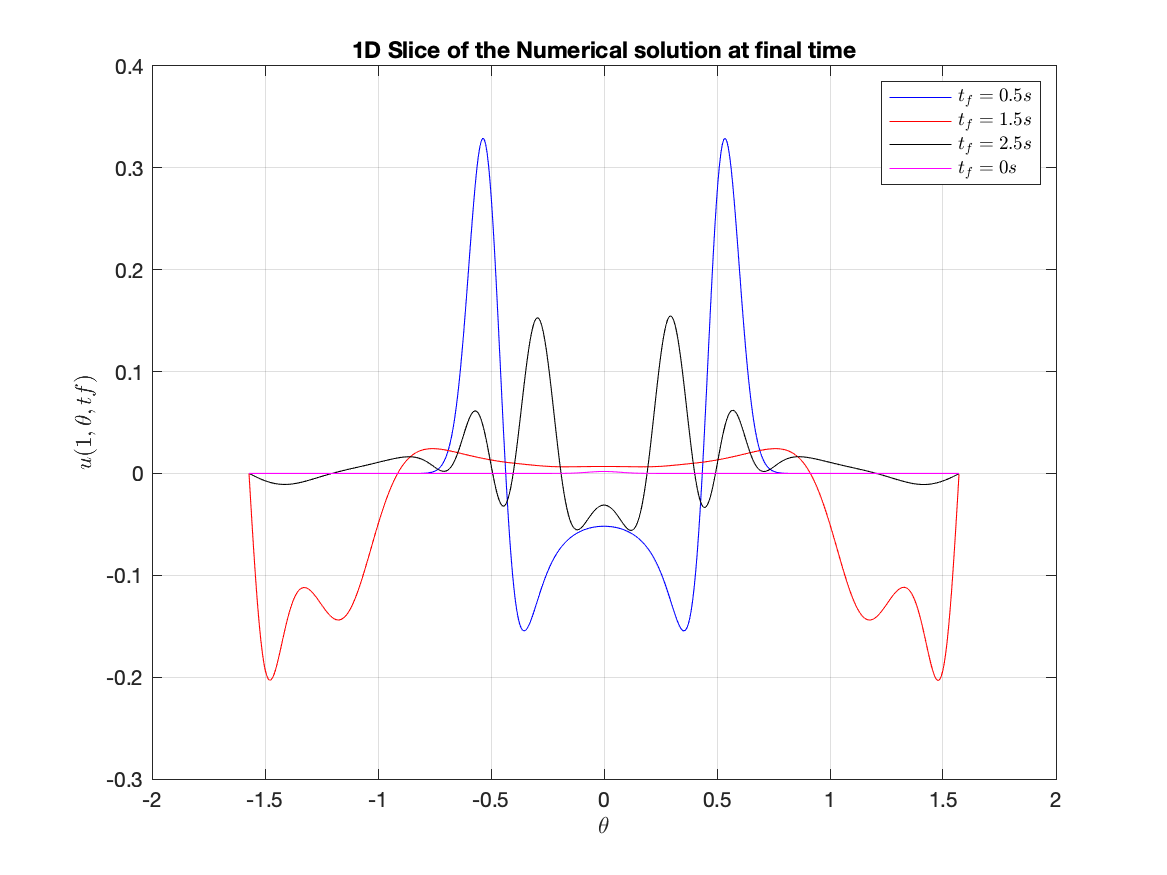
\includegraphics[width=4.2in]{Q2_1Dslice.png}
      \caption{1D slice of the solution at $r=1$}
      \label{fig:Q2_1D}
      \end{figure}
    \end{enumerate}
\end{enumerate}

\vspace{1in}
The following discrete approximations may be useful for problem (1)
\begin{align*}
  u_x(x_j) & = \frac{u_{j+3}-9u_{j+2}+45u_{j+1}-45u_{j-1}+9u_{j-2}-u_{j-3}}{60\Delta x} +O(\Delta x^6)\\
  u_{xx}(x_j) & = \frac{2u_{j+3}-27u_{j+2}+270u_{j+1}-490u_j+270u_{j-1}-27u_{j-2}+2u_{j-3}}{180\Delta x^2} +O(\Delta x^6)\\
  u_{xxx}(x_j) & = \frac{-u_{j+3}+8u_{j+2}-13u_{j+1}+13u_{j-1}-8u_{j-2}+u_{j-3}}{8\Delta x^3} +O(\Delta x^4)\\
  u_{xxxx}(x_j) & = \frac{-u_{j+3}+12u_{j+2}-39u_{j+1}+56u_j-39u_{j-1}+12u_{j-2}-u_{j-3}}{6\Delta x^4} +O(\Delta x^4)\\
  u_{xxxxx}(x_j) & = \frac{u_{j+3}-4u_{j+2}+5u_{j+1}-5u_{j-1}+4u_{j-2}-u_{j-3}}{2\Delta x^5} +O(\Delta x^2)\\
  u_{xxxxxx}(x_j) & = \frac{u_{j+3}-6u_{j+2}+15u_{j+1}-20u_j+15u_{j-1}-6u_{j-2}+u_{j-3}}{\Delta x^6} +O(\Delta x^2)\\
\end{align*}

\end{document}
